\subsection{Data Analysis}

We now want to estimate the dampening constants $\alpha_{1, 2, 3}$ using the resonance curves.
We will show the process of doing that for $\alpha_1$, for the other two it is exactly the same.

The dampening constant $\alpha$ is given as half of the width of the curve at height $A_{\alpha} = A_{max}/\sqrt{2}$.
As we did one measurement per dampening at resonance frequency, this will be our value for $A_{max}$.
To estimate the values of the resonance curve at this height, we make a linear approximation of the curve between the measurement points closest to $A_{\alpha}$.
Then we calculate, where the two resulting linear functions are equal to $A_{\alpha}$.
This gives us the values $\omega_1$ and $\omega_2$.
We now get $\sigma_1 = \omega_0 - \omega_1$ and $\sigma_2 = \omega_0 + \omega_2$.
The dampening constant is then approximated with 
\begin{align*}
	\alpha = \frac{\sigma_1 + \sigma_2}{2}.
\end{align*}
To calculate the error of this value, we perform basically the same calculations as before, once for the upper limit of our error range for the resonance curve and once for the lower limit, as indicated in Fig.\ref{fig::res_calc}.
\begin{figure} [ht]
	\centering
	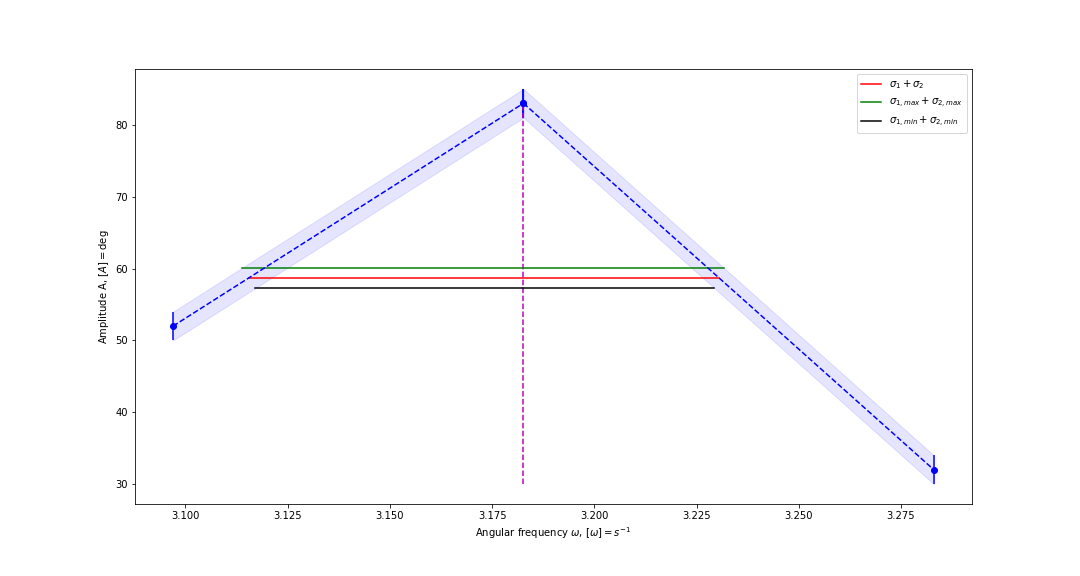
\includegraphics[width=500pt]{python/res_calc.PNG}
	\caption{Important part of resonance curve for dampening $1$. The horizontal lines are the geometrical representation of how $\alpha$ and $\Delta \alpha$ are calculated.}
	\label{fig::res_calc}
\end{figure}

In the end, this leaves us with the following values for $\alpha_{1, 2, 3}$:

\begin{table}[ht]
	\begin{tabularx}{\textwidth}{XM{1.8cm}M{2cm}M{2cm}M{2cm}M{2cm}M{2cm}}%{XXXXXX}{M{1.7cm}M{1.5cm}M{1.5cm}M{2.5cm}M{2cm}}
		\toprule 
		\textbf{$\alpha_{1, 2, 3}$}& \textbf{Value} (\si{\second^{-1}})  & \textbf{Error} \qquad (\si{\second^{-1}}) \\
		\hline
		&&&&&&\\[-5pt]
		$\alpha_1$	& 0.058	& $\pm 0.001$	\\[5pt]
		
		$\alpha_2$	& 0.104 & $\pm 0.003$	\\[5pt]
		
		$\alpha_3$	& 0.160 & $\pm 0.01$	\\[5pt]
		
		\bottomrule 
	\end{tabularx}
	\caption{Table with the measured weights and lengths of the used disc and beams in the experiment. (The length of the disc is the radius of the disk)}
	\label{tab::measure}
\end{table}



